\section*{Pregunta 6}
\noindent Let $P$ be a set of $n$ points in the plane. The staircase of $P$ is the set of all points in the plane that have at least one point in $P$ both above and to the right.
\begin{center}
    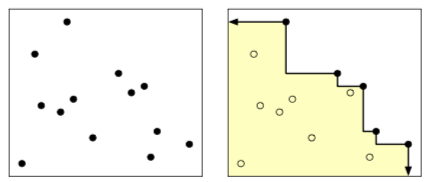
\includegraphics[scale=0.5]{escalera1}
\end{center}

\begin{enumerate}
    \item Describe an algorithm to compute the staircase of a set of $n$ points in $O(n \log n)$ time.
    
    \item Describe and analyze a data structure that stores the staircase of a set of points, and an algorithm ABOVE? $(x, y)$ that returns \textsc{true} if the point $(x, y)$ is above the staircase, or \textsc{fals} otherwise. Your data structure should use $O(n)$ space, and your ABOVE? algorithm should run in $O(log n)$ time.
\end{enumerate}

\begin{center}
    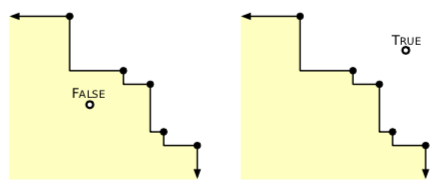
\includegraphics[scale=0.5]{escalera2}
\end{center}

\subsection*{Respuesta}
\begin{enumerate}
    \item Describe an algorithm to compute the staircase of a set of $n$ points in $O(n \log n)$ time.
    \begin{algorithmic}[1]
        \State escalera=$\{\}$
        \State Ordenar los puntos con respecto a $y$
        \State Sacar el primer punto $MAX_y = y(p_1)$
        \State Comparar los puntos $p_j$ tal que $y$ de $p_j$ sea igual a $y$ de $MAX_y$ y tomar de los puntos el que tenga la $x$ mayor (este es el punto más a la derecha) asignarlo como $MAX_x$ 

        \For{$p_i$ en $P$}
        \If{$x(p_i)<MAX_x$} //¿Es punto máximo con respecto a $x$?
            \State //no, entonces
            \State  Sacar el máximo punto actual $MAX_y = p_i$
            \State Comparar los puntos $p_j$ tal que $y$ de $p_j$ sea igual a $y$ de $MAX_y$ y tomar de los puntos el que tenga la $x$ mayor (este es el punto más a la derecha) asignarlo como $MAX_x$ 
        \Else{$\ x(p_i) \geq MAX_x$} // sí, es el maximo
            \State escalera.add($p_i | x=MAX_x \&\& MAX_y$)
        \EndIf
        \EndFor
    \end{algorithmic}

        En este algoritmo nos interesa ordenar los elementos con respecto de $y$ (lo que toma $O(n \log n)$) y luego escoger el punto dentro de las $y$ más grandes donde la $x$ sea la mayor (lo que toma $O(n)$). De esta forma escoger "la altura" del escalon usando $y$ y luego "la anchura" del escalon usado $x$ para que todos los puntos del plano tengan un punto arriba (tomamos el punto más arriba es decir el mayor con respecto de $y$) y a la derecha (tomamos el punto más a la derecha es decir el mayor con respecto de $x$). Y la complejidad del algoritmo queda $O(n+n \log n)\rightarrow O(n \log n)$
    
    \item Describe and analyze a data structure that stores the staircase of a set of points, and an algorithm ABOVE? $(x, y)$ that returns \textsc{true} if the point $(x, y)$ is above the staircase, or \textsc{fals} otherwise. Your data structure should use $O(n)$ space, and your ABOVE? algorithm should run in $O(\log n)$ time.
    
    Podemos utilizar un árbol binario de busqueda y mantenerlo ordenado con respecto a $y$ de forma que si tenemos que desplazarnos en la busqueda hacia arriba o abajo el último nodo accedido se convierte en la raíz lo que acelerara nuestra busqueda. En clase vimos que estos árboles utilizan $O(n)$ en espacio dado que solo es necesario almancenar $n$ nodos.

    Propongo el siguiente algoritmo ABOVE($tree,punto(x,y)$): 
    Notar que si $p$ esta en la escalera entonces $\forall z$ punto en la escalera, se cumple que $x < x(z)$ porque si esto fuera falso implicaría que existe un punto en $P$ que no tiene un punto a la derecha.
    \begin{algorithmic}[1]
        \State $m \gets$ raíz
        \If{$y == y(m)$} //¿El punto esta a la altura de $m$?
            \If{$x \geq x(m)$} //¿El punto esta más a la derecha que $m$?
                \State
                \Return True
                \State //Sí, entonces esta fuera de la escalera
            \Else
                \State
                \Return False
                \State //No, entonces esta en la escalera
            \EndIf
        \EndIf


        \If{$y > y(m)$} //¿El punto esta arriba de $m$?
            \If{¿$m$ es el mayor elemento (la raiz) en el árbol original?}\\
                \Return True//Esta arriba de la escalera
            \Else
                \If{$x \leq m(x)$} //¿El punto esta más a la izquierda que $m$?\\
                    \Return False // Sí,entonces no esta arriba de la escalera
                \Else{$ \ x > m(x)$}
                    \State // No, entonces busca en el subárbol derecho
                    \State ABOVE($rightTree,p(x,y)$)
                \EndIf
            \EndIf
        \EndIf

        \If{$y < y(m)$} //¿El punto esta abajo de $m$?
            \If{¿$m$ es una hoja?}\\
                \If{$x \leq m(x)$} //¿El punto esta más a la izquierda que $m$?\\
                    \Return False // Sí,entonces no esta arriba de la escalera
                \Else{$ \ x > m(x)$}//¿El punto esta más a la derecha que $m$?\\
                    \Return True
                \EndIf
            \Else
                \State //no, entonces busca en el subárbol izquierdo
                \State ABOVE($leftTree,p(x,y)$)
            \EndIf
        \EndIf
    \end{algorithmic}

    La idea es observar por cada escalon (marcado por una $y$ y $x$ que nos indica la altura y la anchura) y observar si el punto esta fuera de todos los escalones: la $y$ nos indica si esta abajo o arriba del escalon y la $x$ si esta dentro del escalon (a la izquierda) o no (esta a la derecha). Como utiliza una modificación de la búsqueda binaria (buscando en cada subárbol) la complejidad del algoritmo es $O(\log n)$
\end{enumerate}
\bigskip
